\documentclass[letterpaper,10pt,conference]{ieeeconf}

\IEEEoverridecommandlockouts
\overrideIEEEmargins

% In case the PDF conversion filter reports corruption/parsing errors,
% uncomment one of the following lines if needed.
% \pdfobjcompresslevel=0
% \pdfminorversion=4

% Packages required by the current paper.
\usepackage[T1]{fontenc}
\usepackage{times}
\usepackage{amsmath}
\usepackage{amssymb}
\usepackage{graphicx}
\usepackage{xcolor}
\usepackage[caption=false,font=footnotesize]{subfig}
\usepackage{float}
\usepackage{booktabs}
\usepackage{multirow}
\usepackage{siunitx}
\usepackage{placeins}
\usepackage{stfloats}
\usepackage{tikz}
\usetikzlibrary{arrows.meta}
\setlength{\textfloatsep}{6pt plus 1pt minus 2pt}
\setlength{\floatsep}{5pt plus 1pt minus 1pt}
\setlength{\intextsep}{6pt plus 1pt minus 2pt}
\setlength{\dbltextfloatsep}{6pt plus 1pt minus 2pt}
\setlength{\dblfloatsep}{5pt plus 1pt minus 1pt}
\usepackage[ruled,vlined,linesnumbered,noend]{algorithm2e}
\usepackage[bookmarks=true,hidelinks]{hyperref}

\newif\ifanonymous

% INTERNAL WRITING / OVERLEAF REVIEW:
% \anonymousfalse
%
% DOUBLE-blind SUBMISSION:
% \anonymoustrue

% Current internal default:
\anonymousfalse

% SELECTED TITLE FOR V1 FRONT-half ALIGNMENT
\newcommand{\papertitle}{RoSC: Role-shared Semantic Coordination for Dynamic
Heterogeneous Multi-arm Manipulation}

\newcommand{\paperauthornames}{}
\newcommand{\paperaffiliation}{}
\newcommand{\papercontact}{}

% Revision markup renders normally unless a review root overrides it.
\providecommand{\update}[1]{#1}


\title{\textbf{\papertitle}}
\author{}

\hypersetup{
  pdftitle={\papertitle},
  pdfauthor={}
}

\begin{document}

\maketitle
\thispagestyle{empty}
\pagestyle{empty}

\begin{abstract}
Heterogeneous multi-arm manipulation can combine complementary workspaces,
end-effectors, and sensing capabilities for concurrent task execution in
dynamic workspaces. However, semantic coordination becomes difficult when the
physical scene changes continually while task-relevant updates, external
disturbances, and execution failures occur only at discrete moments. Static or
monolithic semantic coordination can either miss these events or trigger
unnecessary global replanning that interrupts still-valid execution. This work
addresses this problem through role-shared semantic coordination for dynamic
heterogeneous multi-manipulator scenarios. The framework assigns explicit
semantic responsibilities to the affordance, planning, and verification roles
over a shared semantic state that stores the current instruction, the
assignment-aware primitive graph, task-relevant scene facts, and execution
status. An event-driven selective semantic update procedure further identifies
the affected scope caused by a task update, external disturbance, or execution
failure, and revises only that scope while preserving unaffected valid
execution. Simulation baselines, failure analysis, and ablations show that
explicit responsibility separation reduces coordination errors and selective
semantic updates enable faster adaptation in evolving environments; hardware
trials examine the same mechanisms on a heterogeneous multi-arm platform.
\end{abstract}

\section{Introduction}
\label{sec:introduction}

\providecommand{\introchange}[1]{#1}
\providecommand{\structurechange}[1]{#1}
\providecommand{\localexecchange}[1]{#1}

Heterogeneous multi-manipulator systems must maintain a consistent task
interpretation while complementary robots execute concurrently in a changing
workspace. Figure~\ref{fig:scenario} instantiates this problem with a conveyor
and three task-relevant semantic events. Language- and vision-language-based
grounding~\cite{huang2023inner,liang2023code,rana2023sayplan} does not expose
team capability constraints or
responsibility interfaces; independent agents can therefore maintain
incompatible task views. The challenge is to
establish one capability-aware semantic authority across robots and revise only
the semantics invalidated by a new instruction, disturbance, or verified
failure while local controllers remain responsive to continuous scene
evolution. We propose RoSC, a role-shared semantic coordination framework with
an event-driven selective update that follows event detection $\rightarrow$
affected-scope selection $\rightarrow$ semantic-state revision $\rightarrow$
continued dispatch from a consistent frontier. Simulation baselines, failure
analysis, and mechanism ablations test these mechanisms, while hardware trials
check the same update sequence during physical execution.

\begin{figure}[t]
    \centering
    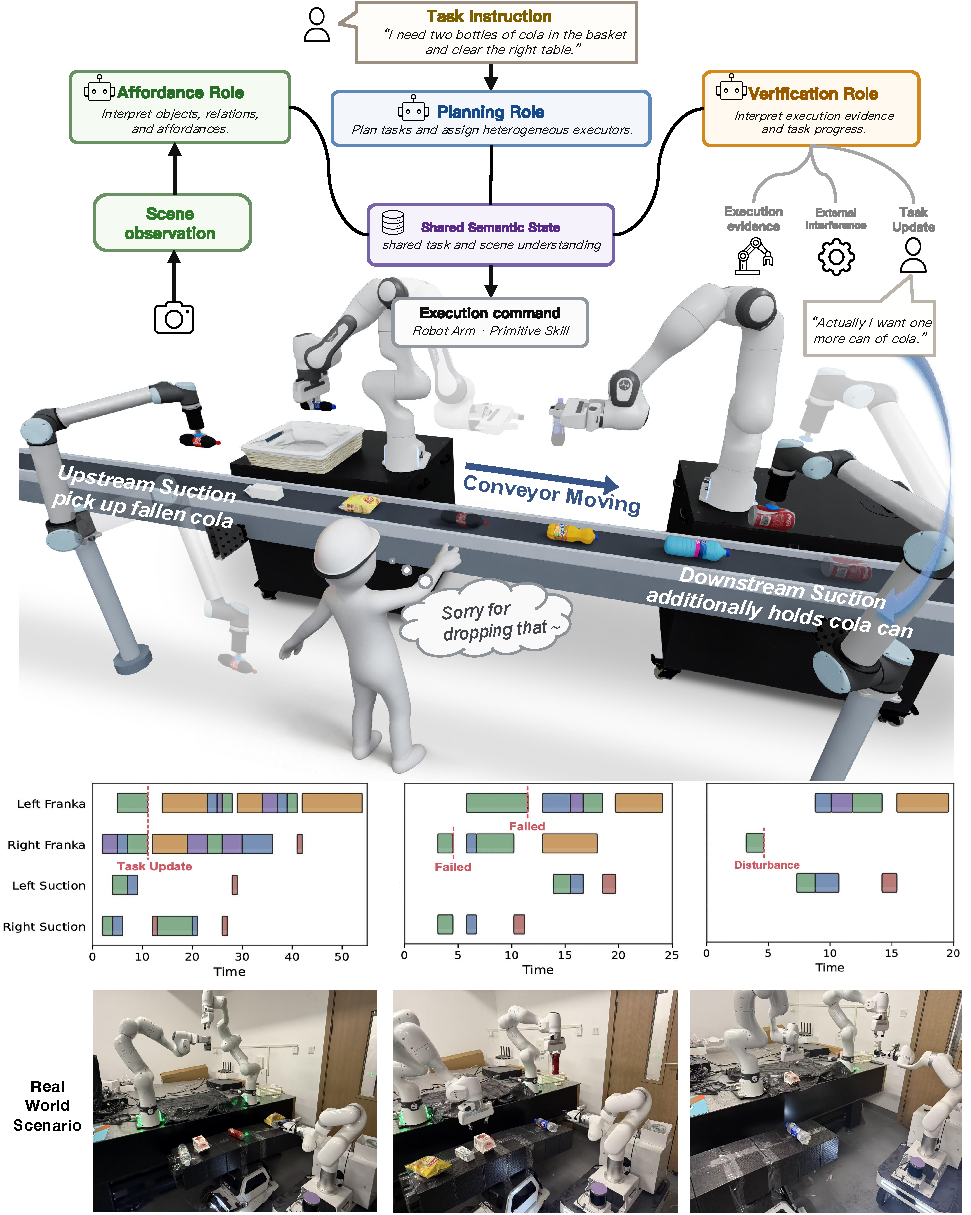
\includegraphics[width=\columnwidth]{figures/figure1_final_lowercase.pdf}
    \caption{The shared semantic state coordinates three roles while preserving
    local execution. \textbf{Top:} framework and simulated conveyor workspace;
    \textbf{Middle:} event Gantt charts; \textbf{Bottom left:} normal hardware
    execution; \textbf{Bottom middle:} hardware task update; \textbf{Bottom
    right:} hardware external disturbance.}
    \label{fig:scenario}
\end{figure}

\begin{figure*}[!t]
  \centering
  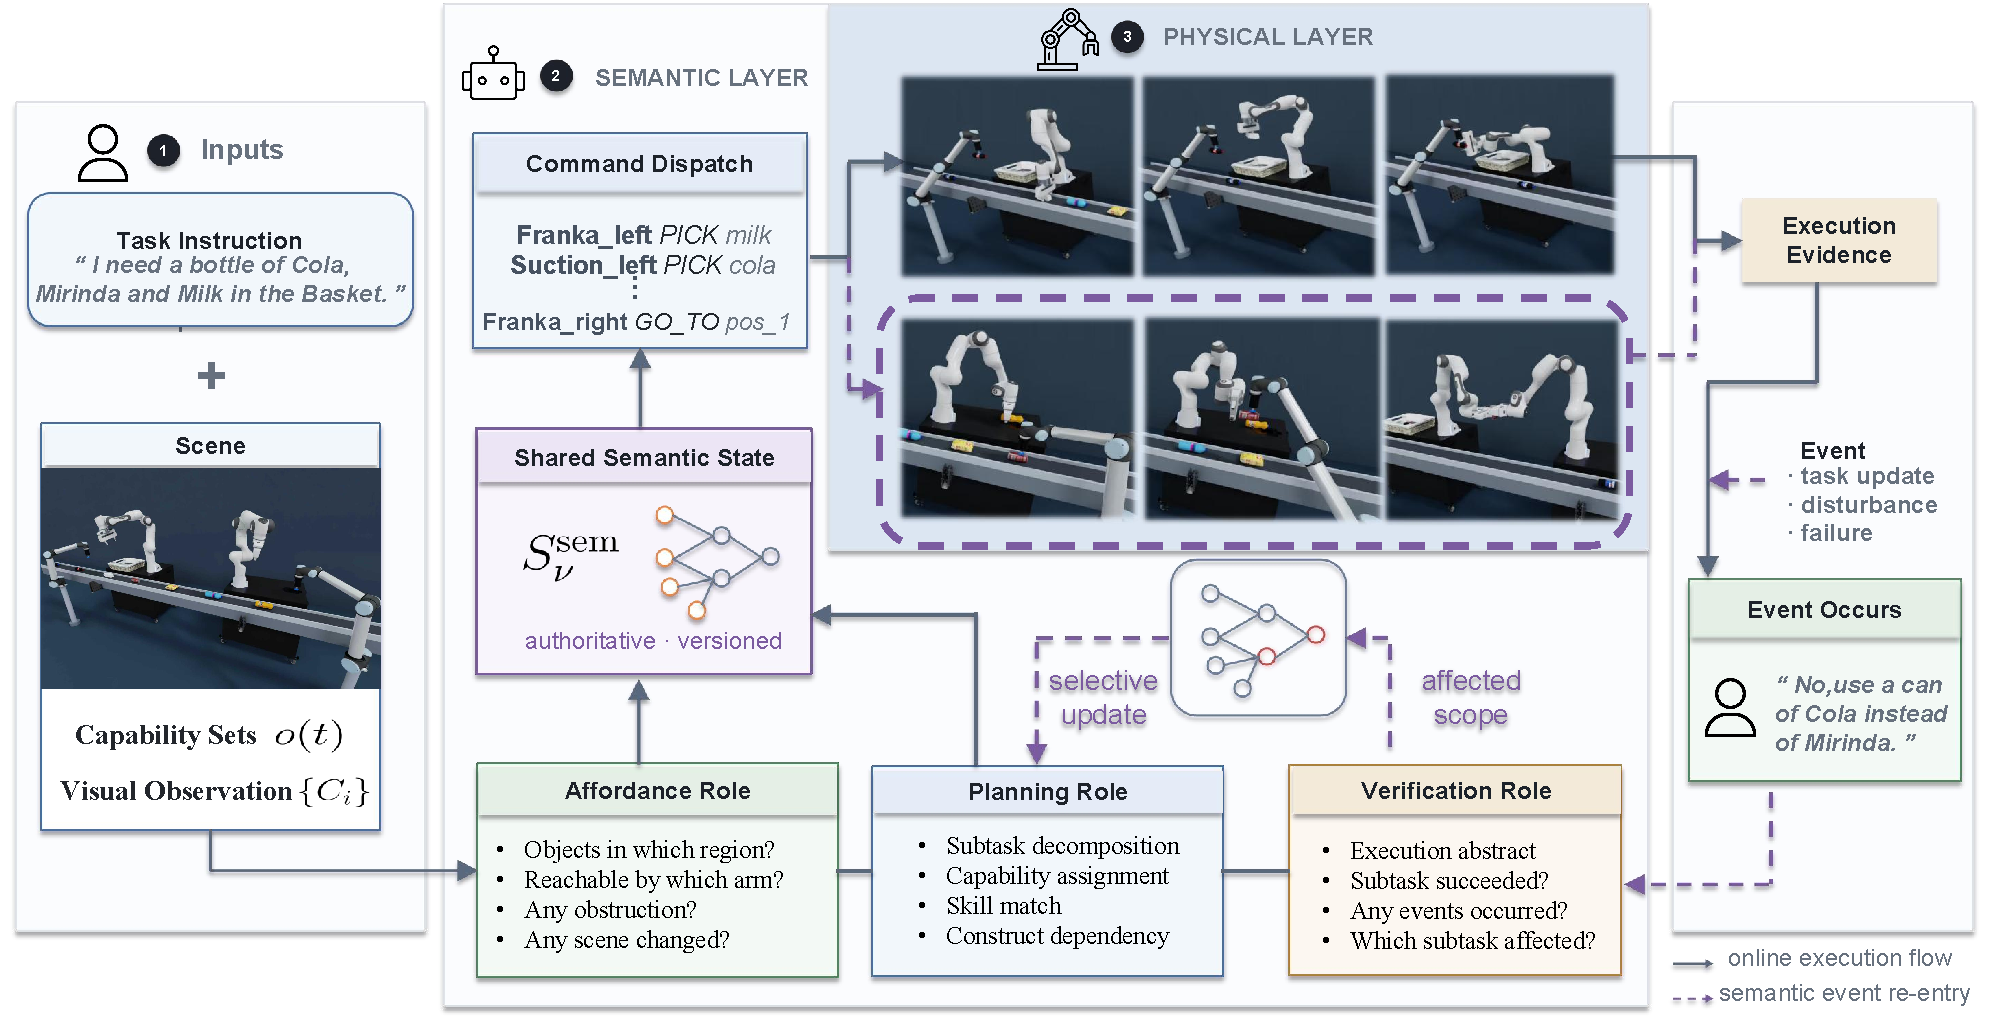
\includegraphics[width=0.96\textwidth]{figures/figure2.pdf}
  \caption{Role-shared coordination links semantic decisions to physical
  execution. Affordance evaluates scene feasibility; planning decomposes and
  assigns subtasks, skills, and dependencies; verification abstracts execution
  evidence, checks outcomes and events, and identifies affected subtasks. Solid
  and dashed arrows denote online execution and selective event updates.}
  \label{fig:method_overview}
\end{figure*}

\subsection{Related Work}
\label{sec:related_work}
\providecommand{\finalchange}[1]{#1}
\providecommand{\localexecchange}[1]{#1}

Language-guided grounding methods translate natural-language instructions into
spatial representations, executable programs, or scene-grounded task
plans~\cite{huang2023inner,liang2023code,rana2023sayplan,
huang2023voxposer}. Building on these capabilities, LLM-based multi-robot
frameworks adopt different coordination structures: RoCo uses inter-robot
dialogue; COHERENT relies on centralized proposals and execution feedback;
MALLVI reactivates specialized agents when needed; and CoMuRoS and DEXTER-LLM
revise tasks or assignments in response to events~\cite{
mandi2024roco,liu2025coherent,taji2026mallvi,
borate2026comuros,zhu2025dexter}. Other systems explicitly incorporate
capability-aware coalitions, dependency-based task allocation, or separate
planning, manipulation, and verification agents~\cite{
kannan2024smartllm,obata2025lipllm,he2026closedloop}. Collectively, these
methods establish effective mechanisms for grounding, agent interaction, and
task revision, but they do not explicitly organize ownership of the distinct
semantic components that must remain consistent as multiple heterogeneous
manipulators execute concurrently. RoSC addresses this issue by maintaining
the authoritative shared state and assigning responsibility
to the affordance, planning, and verification
roles, respectively. When a discrete semantic event occurs, these roles
identify its dependency-closed affected scope and reconstruct only the
invalidated subgraph, while preserving unaffected valid execution and leaving
continuous physical adaptation to the local controllers.


Dynamic manipulation supports tracked or reactive grasping and visual
servoing~\cite{marturi2019dynamic,maranci2026reactive,liu2023target,
haviland2020finalphase}, allowing local controllers to continuously adapt
end-effector motion to moving targets and perception updates. Execution
monitoring and continual replanning further address runtime deviations by
detecting discrepancies between expected and observed outcomes and invoking
recovery or plan revision~\cite{pettersson2005execution,brenner2009continual,
levihn2013foresight,pezzato2023active}. These methods primarily focus on
maintaining physical feasibility, monitoring action execution, or revising a
plan after deviations. However, in heterogeneous multi-manipulator settings,
the resulting feedback may affect different parts of the team-level semantic
state: a new observation may change an object's affordance, a failed action may
invalidate its execution status and downstream dependencies, and a revised
instruction may alter only one task branch. RoSC explicitly separates these
responsibilities among affordance, verification, and planning roles. It uses
the shared semantic state to determine which information must be refreshed,
which subtasks are affected, and whether planning should be invoked, thereby
supporting event-scoped semantic revision while preserving unaffected valid
execution.


\subsection{Our Method}
\label{sec:our_method_intro}

Figure~\ref{fig:method_overview} shows the resulting framework. At task start,
the affordance role evaluates object regions, reachability, obstructions, and
scene changes to produce $\mathcal{F}$; the planning role decomposes the task,
matches skills and capabilities to manipulators, constructs $G$, and initializes
the versioned shared semantic state
$S_\nu^{\texttt{sem}}=(\gamma,G,\mathcal{F},z)$. The framework then selects the
verified executable frontier, constructs capability-valid commands, and
dispatches independent commands concurrently to the assigned manipulators.
After local execution, affordance refreshes $\mathcal{F}$ and verification
abstracts the evidence, checks the outcome, updates $z$, and detects events. For
an event, verification identifies $\mathcal{N}_k^{\texttt{aff}}$; planning
replans that subgraph while preserving valid work outside it, then dispatch
continues from the updated frontier. This restricted semantic update shortens
the response path and helps preserve opportunities as the scene evolves.

The main contribution of this work is twofold: (I) A role-shared semantic
coordination formulation is introduced for dynamic heterogeneous
multi-manipulator scenarios with continual physical changes, assigning explicit
responsibility to the affordance, planning, and verification roles; and (II) An
event-driven selective semantic update procedure is developed to efficiently
handle task updates, external disturbances, and execution failures while
preserving unaffected valid execution.

\section{Problem Formulation}
\label{sec:formulation}

\providecommand{\structurechange}[1]{#1}
\newtheorem{problem}{Problem}

\subsection{Heterogeneous Manipulator Team}
\label{sec:system_description}

Consider a team of heterogeneous robotic manipulators
\begin{equation}
 \mathcal{R}\triangleq\{r_i\}_{i=1}^{N},
 \label{eq:manipulator_team}
\end{equation}
where the team in~\eqref{eq:manipulator_team} contains $N$ manipulators and
$r_i$ has capability set
$\mathcal{C}_i$. A capability set describes the primitive actions, targets,
and embodiment conditions available to the corresponding manipulator. The
system receives a natural-language task $\gamma$ and continuous visual
observations $o(t)$ while the physical workspace evolves.

The execution process can also produce discrete semantic events
\begin{equation}
 e_k\in\mathcal{E}\triangleq
 \{e^{\texttt{t}},e^{\texttt{x}},e^{\texttt{f}}\},
 \label{eq:semantic_events}
\end{equation}
where $e^{\texttt{t}}$ denotes an online task update, $e^{\texttt{x}}$ denotes
an external disturbance, and $e^{\texttt{f}}$ denotes an execution failure.
Continuous physical motion, including motion of a target on a conveyor, remains
part of the evolving workspace and is not itself a semantic event.

\subsection{Online Primitive Command Sets}
\label{sec:online_commands}

An executable command $c$ is an instruction that can be sent directly to a
manipulator execution interface. It specifies, through the interface
representation rather than a semantic graph node, the execution skill, semantic
target or object, and manipulator that executes the skill. Thus, a semantic
subtask or graph node is not itself a command; the required output is an online
sequence of command sets
\begin{equation}
 \mathbf{C}\triangleq
 (\mathbf{c}_1,\mathbf{c}_2,\cdots,\mathbf{c}_M),
 \label{eq:command_sequence}
\end{equation}
where $M$ is determined online, each $\mathbf{c}_m$ contains capability-valid
commands that can be issued concurrently to the team, and the internal command
fields are defined in Section~\ref{sec:construct_commands}. The next command
set is generated online by the role-shared coordination
pipeline from the task, heterogeneous capabilities, visual history, semantic
event history, and previously issued command sets:
\begin{equation}
 \mathbf{c}_m=
 \Pi_{\mathrm{coord}}\!\left(
 \gamma,\{\mathcal{C}_i\}_{i=1}^{N},o(0\!:\!t_m),
 e_{1:k_m},\mathbf{c}_{1:m-1}\right),
 \label{eq:online_command_generation}
\end{equation}
where $t_m$ is the decision time and $k_m$ is the number of semantic events
observed by that time. The operator $\Pi_{\mathrm{coord}}$ in
\eqref{eq:online_command_generation} denotes the
complete online pipeline whose internal stages construct the dependency graph
$G$, executable commands, and verification status as defined
in the Method. The ordering of the arguments preserves the information flow
from task specification and embodiment capabilities to observations, events,
and prior command sets.

\subsection{Online Coordination Problem}
\label{sec:coordination_problem}

The physical workspace may change continuously between decision times, and the
event stream may contain task updates, external disturbances, or execution
failures. The command sequence must support concurrent progress while
respecting each manipulator's capability set and the dependencies induced by the
task. No scalar optimization objective is imposed in this formulation; the
primary requirement is completion of the current task under the stated online
information and execution conditions.

\begin{problem}
Given a natural-language task $\gamma$, a heterogeneous team $\mathcal{R}$ with
capability sets $\{\mathcal{C}_i\}_{i=1}^{N}$, continuous visual observations
$o(t)$, and the event history in~\eqref{eq:semantic_events}, compute the online
command-set sequence $\mathbf{C}$ in~\eqref{eq:command_sequence} such that
the primitive commands are capability-valid, independent commands can execute
concurrently, and the current task is completed despite continuous physical
evolution and the possible occurrence of $e^{\texttt{t}}$, $e^{\texttt{x}}$,
or $e^{\texttt{f}}$.\hfill $\blacksquare$
\end{problem}

\section{Method}
\label{sec:proposed_solution}

This section presents the role-shared semantic coordination framework shown in
Figure~\ref{fig:method_overview}. Its three roles respectively evaluate scene
feasibility, decompose and assign task dependencies, and verify outcomes while
identifying event-affected subtasks. Section~\ref{sec:role_shared_coordination}
defines the shared semantic state and these three responsibilities,
Section~\ref{sec:semantic_physical_coordination} describes event-scoped
updates, Section~\ref{sec:dispatch_execute} constructs and verifies executable
commands, and Section~\ref{sec:closed_loop_coordination} gives the online
algorithm and complexity discussion.

\subsection{Construct the role-shared semantic state}
\label{sec:role_shared_coordination}

The shared semantic state is the authoritative task-level state maintained by
the three semantic roles during the current coordination cycle:
\begin{equation}
 S_\nu^{\texttt{sem}}\triangleq
 \bigl(\gamma,G,\mathcal{F},z\bigr),
 \label{eq:semantic_state}
\end{equation}
where $\nu$ is the semantic version, $\gamma$ is the current task instruction,
$G$ is the assignment-aware primitive graph,
$\mathcal{F}$ contains task-relevant scene and feasibility facts, and $z$
records primitive-subtask execution status. This state excludes
manipulator-local control variables and stores only the semantic information
used for task-level coordination.

The affordance role maintains $\mathcal{F}$ through
\begin{equation*}
 \rho_A:o(t)\mapsto\mathcal{F}.
\end{equation*}
It extracts task-relevant scene and
feasibility facts from the observation stream, including object grounding,
relations, affordances, and feasible primitive interactions. During
initialization, observed objects are grounded to semantic targets in
$\gamma$. After each primitive execution, the latest observation refreshes
$\mathcal{F}$ before planning or verification consumes the updated physical
facts.

The planning role maintains $G$ by first deriving an intermediate abstract
dependency graph from $\gamma$ and $\mathcal{F}$, then adding manipulator
assignment and execution dependencies. The final assignment-aware primitive
graph is
\begin{equation}
 \begin{aligned}
 G&=
 \rho_P\!\left(
 \gamma,\mathcal{F},\{\mathcal{C}_i\}_{i=1}^{N},\mathcal{R}\right)\\
 &\triangleq\bigl(\mathcal{N},\mathcal{L}\bigr),
 \end{aligned}
 \label{eq:planning_pipeline}
\end{equation}
where, for each $n\in\mathcal{N}$,
$n\triangleq\bigl(s_n,q_n,r_i,\kappa_n\bigr)$ denotes an assigned primitive
node with primitive skill type $s_n$, semantic target $q_n$, assigned
manipulator $r_i$, and execution skill $\kappa_n$. The relations in
$\mathcal{L}$ include the semantic task dependencies from the intermediate
dependency graph and manipulator-aware dependencies induced by $\mathcal{R}$.
Thus, $G$ records what to execute, who executes it, and which skill
is used. For $n\in\mathcal{N}$,
$\operatorname{pred}(n)$ denotes the predecessor nodes $j$ such that
$(j,n)\in\mathcal{L}$.

The verification role maintains $z$ after command execution. For an executable
command $c_n$, the command sent to the assigned manipulator interface specifies
the required execution skill and semantic target associated with primitive
subtask $n$. After $c_n$ is executed, the latest observation first refreshes
$\mathcal{F}$; the verification role then extracts transient execution
evidence
\begin{equation}
 \eta_n=\rho_V^{\texttt{e}}\bigl(c_n,\mathcal{F}\bigr),
 \label{eq:verification_evidence}
\end{equation}
where $\eta_n$ is the transient execution evidence for the executed command.
The verification role compares evidence with the current instruction to update
status and detect task-relevant events:
\begin{equation}
 \bigl(e_k,z(n)\bigr)=
 \rho_V^{\texttt{z}}\bigl(\eta_n,\gamma\bigr),
 \label{eq:verification_status}
\end{equation}
Here, $z(n)$ is the primitive-subtask status and $e_k$ records any detected
event in~\eqref{eq:semantic_events}; its affected scope is identified in
Section~\ref{sec:semantic_physical_coordination}. Without a task-relevant
inconsistency, $e_k$ is null and only $z(n)$ is updated.

Within $S_\nu^{\texttt{sem}}=(\gamma,G,\mathcal{F},z)$, the affordance,
planning, and verification roles own $\mathcal{F}$, $G$, and $z$, respectively.
An updated $\gamma$ enters as an external semantic constraint and is committed
before role-specific updates. The intermediate graph is used
only to construct $G$, and $\eta_n$ remains transient verification evidence.

\subsection{Event-driven Selective Semantic Updates}
\label{sec:semantic_physical_coordination}

Task-relevant events enter the shared semantic state, whereas continuous
physical evolution remains within manipulator-local execution. Event handling
identifies the invalid scope and invokes adaptation, as shown in
Fig.~\ref{fig:event_graph_update}.

\begin{figure}[t!]
  \centering
  \definecolor{figink}{HTML}{20252A}
\definecolor{figmuted}{HTML}{6B737A}
\definecolor{figpurple}{HTML}{8E5BBE}
\definecolor{figgreen}{HTML}{4D8B55}
\definecolor{figblue}{HTML}{2F6DA6}
\definecolor{figline}{HTML}{D9DDE3}

% Fill one IEEE/ICRA column exactly.  The explicit reset of the TikZ
% bounding box removes the residual left margin introduced by node extents.
\resizebox{\columnwidth}{!}{%
\begin{tikzpicture}[x=1cm,y=1cm,>=Latex]
  \tikzset{
    head/.style={font=\sffamily\bfseries\fontsize{8}{8.8}\selectfont,text=figink},
    subtitle/.style={font=\sffamily\fontsize{8}{8.8}\selectfont,text=figink,align=center},
    eventlabel/.style={font=\sffamily\bfseries\fontsize{8}{8.8}\selectfont,
                       text=figink},
    flow/.style={-Latex,draw=figink!70,line width=.42pt},
    graphpdf/.style={inner sep=0pt,outer sep=0pt}
  }

  % Six graph PDFs are stored under figures/figure3/.
  \def\figpath{figures/figure3}

  % ------------------------------------------------------------
  % Column headers
  % ------------------------------------------------------------
  \node[head] at (1.85,6.82) {$G$};
  \node[head] at (6.94,6.82) {$G'$};

  % ------------------------------------------------------------
  % E1: Task update
  % ------------------------------------------------------------
  \node[graphpdf] at (1.85,5.58)
    {
\includegraphics[width=3.70cm]{\figpath/figure3_E1_Gassign_before.pdf}};
  \draw[flow] (3.73,5.58) -- node[eventlabel,above=2pt] {$e^{\texttt{t}}$} (5.00,5.58);
  \node[graphpdf] at (6.94,5.58)
    {
\includegraphics[width=3.84cm]{\figpath/figure3_E1_Gassign_after.pdf}};
  \node[subtitle,text width=8.56cm] at (4.43,4.50)
    {\textbf{Task update:} the user wants crisps instead of biscuit after $n_4$ is executed.};

  \draw[figline,line width=.35pt] (0.00,4.15) -- (8.86,4.15);

  % ------------------------------------------------------------
  % E2: External disturbance
  % ------------------------------------------------------------
  \node[graphpdf] at (1.85,3.19)
    {
\includegraphics[width=3.70cm]{\figpath/figure3_E2_Gassign_before.pdf}};
  \draw[flow] (3.73,3.19) -- node[eventlabel,above=2pt] {$e^{\texttt{x}}$} (5.00,3.19);
  \node[graphpdf] at (6.94,3.19)
    {
\includegraphics[width=3.84cm]{\figpath/figure3_E2_Gassign_after.pdf}};
  \node[subtitle,text width=8.56cm] at (4.43,2.06)
    {\textbf{External disturbance:} the biscuit is manually taken and placed downstream on the conveyor while $n_5$ is being executed.};

  \draw[figline,line width=.35pt] (0.00,1.72) -- (8.86,1.72);

  % ------------------------------------------------------------
  % E3: Execution failure
  % ------------------------------------------------------------
  \node[graphpdf] at (1.86,0.67)
    {
\includegraphics[width=3.72cm]{\figpath/figure3_E3_Gassign_before.pdf}};
  \draw[flow] (3.75,0.67) -- node[eventlabel,above=2pt] {$e^{\texttt{f}}$} (4.98,0.67);
  \node[graphpdf] at (6.93,0.67)
    {
\includegraphics[width=3.86cm]{\figpath/figure3_E3_Gassign_after.pdf}};
  \node[subtitle,text width=8.60cm] at (4.43,-0.63)
    {\textbf{Execution failure:} $n_1$ fails because the conveyor moves too fast and the Franka misses the grasp; the downstream suction arm prepares in advance for the pick.};

  % Reset the natural node-based bounding box, then define an exact full-column box.
  % This removes the visible blank strip on the left when the input is centered.
  \pgfresetboundingbox
  \path[use as bounding box] (0.00,-0.90) rectangle (8.86,7.02);
\end{tikzpicture}%
}

  \caption{Selective graph transitions
  $G\rightarrow e_k\rightarrow G'$ for task updates, external
  disturbances, and execution failures. Purple contours mark
  $\mathcal{N}_k^{\texttt{aff}}$, unfinished or dependency-invalidated nodes
  requiring reconsideration and reconstruction; failed attempts recorded in
  $z$ need not be reconstructed. Green nodes are retained and blue nodes are new.}
  \label{fig:event_graph_update}
\end{figure}

\subsubsection{Event-affected Scope Identification}
\label{sec:affected_subtasks}

The event types are defined in~\eqref{eq:semantic_events}. A task update
changes the current instruction, an external disturbance is interpreted from
fresh visual evidence, and an execution failure is established by verification.
The event then enters the verification role, which identifies the affected
assignment-aware primitive nodes:
\begin{equation}
 \mathcal{N}_k^{\texttt{aff}}\triangleq
 \rho_V^{\texttt{aff}}\bigl(
 e_k,\gamma,G,\mathcal{F},z\bigr),
 \label{eq:affected_subtasks}
\end{equation}
where $\mathcal{N}_k^{\texttt{aff}}\subseteq\mathcal{N}$
contains the nodes whose task meaning, feasibility, execution status, or
dependencies require reconsideration. The operator tests $e_k$ against the
current $\gamma$, $G$, refreshed $\mathcal{F}$, and verified $z$. Its
event-specific inconsistency checks select requirements invalidated by a task
update, scene-dependent assumptions invalidated by a disturbance, or nodes
marked $\texttt{FAILED}$ after execution. Verification then traces outgoing
dependencies in $G$ to include unfinished descendants whose validity or
executability depends on those nodes, while independent valid nodes remain
outside $\mathcal{N}_k^{\texttt{aff}}$ and are preserved.

\subsubsection{Selective Semantic-state Reconstruction}
\label{sec:update_affected_state}

The selective update produces the next committed semantic state:
\begin{equation}
 S_{\nu+1}^{\texttt{sem}}\triangleq
 \mathcal{U}\!\left(
 S_\nu^{\texttt{sem}},e_k,\mathcal{N}_k^{\texttt{aff}}\right),
 \label{eq:semantic_state_update}
\end{equation}
where $\mathcal{U}$ denotes the final result of the coordinated role updates
rather than a separate replanning step. Before this result is committed, the
affordance role refreshes $\mathcal{F}$, and the verification role updates $z$
and produces $\mathcal{N}_k^{\texttt{aff}}$ by~\eqref{eq:affected_subtasks}.
Using this affected set and the latest $\mathcal{F}$, the planning role retains
exactly the nodes of $G$ outside $\mathcal{N}_k^{\texttt{aff}}$, together with
the relations whose endpoints are both retained. It replans the nodes in
$\mathcal{N}_k^{\texttt{aff}}$, grounds and capability-assigns their
replacements from the updated state, and reconnects the revised subgraph to the
retained graph at the dependency boundary, thereby completing a partial
reconstruction of $G$. The status of each retained node is preserved, whereas
each new or revised node starts as $\texttt{PENDING}$. The reconstructed graph
is checked for capability-valid assignments and predecessor consistency. The
affordance, planning, and verification roles have then respectively updated
$\mathcal{F}$, $G$, and $z$; together with the event-consistent $\gamma$, these
components form $S_{\nu+1}^{\texttt{sem}}$ and advance the semantic version from
$\nu$ to $\nu+1$.

\subsection{Primitive-command Dispatch and Execution}
\label{sec:dispatch_execute}

\subsubsection{Capability-valid Command Construction}
\label{sec:construct_commands}

The command notion  is
instantiated after planning has produced assignment-aware primitive nodes. At
each execution step, $\mathcal{N}_{\texttt{exec}}$ is the temporary set of
executable primitive subtasks in $G$. A node $n$
belongs to $\mathcal{N}_{\texttt{exec}}$ when
$z(n)\ne\texttt{COMPLETE}$ and $z(n')=\texttt{COMPLETE}$ for every
$n'\in\operatorname{pred}(n)$. For any
$n\in\mathcal{N}_{\texttt{exec}}$, command construction is given by:
\begin{equation}
 c_n=\phi_C(n),
 \qquad
 \phi_C:\mathcal{N}_{\texttt{exec}}\rightarrow\mathcal{C},
 \label{eq:execution_command}
\end{equation}
where $\phi_C$ is the command construction function and $\mathcal{C}$ denotes
the executable command space, distinct from the per-manipulator capability
sets $\{\mathcal{C}_i\}_{i=1}^{N}$. Although $n$ contains semantic execution
information, $c_n$ is the executable command sent to the robot interface. At
each execution step, the commands generated from
$\mathcal{N}_{\texttt{exec}}$ form a concurrent command set
$\mathbf{c}_m=\{c_{n_1},c_{n_2},\cdots\}$.

\subsubsection{Local Execution and Outcome Verification}
\label{sec:manipulator_local_execution}

The assigned local skill executes each command using the manipulator's current
perception, tracking, and control stack. Its target reference allows continuous
motion to remain local. After execution, the latest observation refreshes
$\mathcal{F}$ through $\mathcal{F}\gets\rho_A(o_t')$ without semantic
replanning. For each executed command, verification extracts $\eta_n$ via
\eqref{eq:verification_evidence} and uses $(\eta_n,\gamma)$ to update $z(n)$ and
detect any $e_k$ via~\eqref{eq:verification_status}. A detected event triggers
identification and selective state revision.

\subsection{Closed-Loop Coordination}
\label{sec:closed_loop_coordination}

\subsubsection{Online Coordination Algorithm}

Algorithm~\ref{alg:coordination} summarizes the online procedure. At task start,
the affordance role observes the scene and extracts $\mathcal{F}$. The planning
role then derives the task dependencies, constructs the assignment-aware $G$,
and initializes $S_\nu^{\texttt{sem}}=(\gamma,G,\mathcal{F},z)$. During each
loop, the verified frontier selects independent executable nodes, maps them to
capability-valid commands, and dispatches the concurrent command set to the
assigned manipulators. After local execution, affordance refreshes
$\mathcal{F}$; for every executed command, verification extracts $\eta_n$ and
uses $(\eta_n,\gamma)$ to update $z(n)$ and detect any $e_k$. When an event
occurs, verification reads the refreshed $\mathcal{F}$ together with
$e_k$, $\gamma$, $G$, and $z$, applies the event-specific criterion and traces
unfinished dependent nodes, and outputs $\mathcal{N}_k^{\texttt{aff}}$. The
planning role then retains the nodes outside this set, replans only the affected
nodes using the latest $\mathcal{F}$, and reconnects the revised subgraph. The
three role updates are committed as $S_{\nu+1}^{\texttt{sem}}$, after which
dispatch resumes from the new consistent frontier. Restricting recomputation to this
dependency-closed scope is intended to shorten semantic-event response time and
reduce the chance that ongoing physical evolution removes an available
manipulation opportunity.

\begin{algorithm}[t!]
\caption{Online role-shared semantic coord.}
\label{alg:coordination}
\KwIn{$\gamma$, $o(t)$, $\{\mathcal{C}_i\}_{i=1}^{N}$, $\mathcal{R}$}
\KwOut{$\mathbf{C}$}

Extract $\mathcal{F}$ from $o(0)$\;
Construct $G$ by~\eqref{eq:planning_pipeline}\;
Initialize $S_\nu^{\texttt{sem}}$ by~\eqref{eq:semantic_state};
$\mathbf{C}\gets()$\;

\While{task incomplete}{
    $\mathcal{N}_{\texttt{exec}}\gets
    \{n\in\mathcal{N}\mid z(n)\ne\texttt{COMPLETE},
    \ z(n')=\texttt{COMPLETE},\
    \forall n'\in\operatorname{pred}(n)\}$\;

    $\mathbf{c}_m\gets
    \{c_n\mid n\in\mathcal{N}_{\texttt{exec}}\}$
    using~\eqref{eq:execution_command}\;
    Append $\mathbf{c}_m$ to $\mathbf{C}$ and execute it\;
    Refresh $\mathcal{F}$ from $o_t'$\;

    \ForEach{$c_n\in\mathbf{c}_m$}{
        Extract $\eta_n$ by~\eqref{eq:verification_evidence}\;
        Update $(e_k,z(n))$ by~\eqref{eq:verification_status}\;
    }

    \If{$e_k$ is detected}{
        Identify $\mathcal{N}_k^{\texttt{aff}}$
        by~\eqref{eq:affected_subtasks}\;
        Retain $G\setminus\mathcal{N}_k^{\texttt{aff}}$ and reconstruct
        the affected subgraph using $\mathcal{F}$\;
        Commit $S_{\nu+1}^{\texttt{sem}}$
        by~\eqref{eq:semantic_state_update};
        $\nu\gets\nu+1$\;
    }
}
\end{algorithm}

\subsubsection{Event-specific Coordination}
\label{sec:event_specific_algorithm}

The same protocol handles all events. For $\texttt{E1}$, verification marks the
requirement-changing branch and planning regenerates only that branch. For
$\texttt{E2}$, refreshed $\mathcal{F}$ invalidates nodes whose target,
feasibility, or dependency assumptions changed. For $\texttt{E3}$, the failed
node and unfinished downstream descendants receive a  repair
branch. Valid completed nodes, independent pending work, and local tracking are
retained. Thus, affordance supplies current facts, verification selects scope,
and planning revises only the invalidated semantic subgraph.

\subsubsection{Computational Complexity}

The explicit graph operations in Algorithm~\ref{alg:coordination} are linear
in the maintained graph when predecessor lists are stored with the graph.
Checking executable nodes requires scanning $\mathcal{N}$ and the relevant
incoming dependencies, with worst-case cost $O(|\mathcal{N}|+|\mathcal{L}|)$ per
dispatch step. After an event, selective revision is bounded by the affected
subgraph identified by $\mathcal{N}_k^{\texttt{aff}}$ and its incident
dependencies. The complexity of the semantic operators
$\rho_P$, $\rho_V^{\texttt{e}}$,
$\rho_V^{\texttt{z}}$, and $\rho_V^{\texttt{aff}}$ also includes the call time
of the concrete LLM/VLM models used by these operators. Because these call
times depend on the selected models and serving conditions, no closed-form
bound is assigned here.

\providecommand{\expplaceholder}{\textbf{***}}

\section{Experiments}
\label{sec:experiments}

This section tests whether role-shared semantic coordination improves task
correctness, preserves useful concurrent execution, and limits event-driven
updates to invalidated work. Simulation compares the proposed method with
three matched baselines over static, dynamic, and event conditions. Failure
counts and mechanism ablations then localize the source of the differences.
Hardware trials provide a physical check of the same semantic-state update
sequence.

\begin{figure}[t!]
  \centering
  \setlength{\tabcolsep}{3pt}
  % Equal-height cells align both columns while preserving each PDF aspect ratio.
  \newcommand{\ganttpanel}[1]{%
    \parbox[c][.93in][c]{.485\columnwidth}{\centering
      \includegraphics[width=.485\columnwidth]{#1}}}
  % The trajectory PDFs are shorter than their paired Gantt charts; lower
  % them slightly so the three row pairs share a common lower edge.
  \newcommand{\ganttpanelleft}[1]{%
    \parbox[c][.93in][c]{.485\columnwidth}{\centering
      \raisebox{+0.15in}{\includegraphics[width=.485\columnwidth]{#1}}}}
  \newcommand{\ganttrlabel}[1]{%
    \llap{\raisebox{.46in}{\textbf{(#1)}\hspace{2pt}}}}
  % Compact semantic-role response strip for each event row.
  \definecolor{g4affline}{HTML}{3E8050}
  \definecolor{g4afffill}{HTML}{F2F8F3}
  \definecolor{g4verline}{HTML}{B56A16}
  \definecolor{g4verfill}{HTML}{FFF8ED}
  \definecolor{g4planline}{HTML}{356FA8}
  \definecolor{g4planfill}{HTML}{F1F6FB}
  \newcommand{\rolechip}[5]{%
    \node[draw=#1,fill=#2,rounded corners=1.5pt,line width=0.45pt,
      minimum width=.285\columnwidth,text width=.265\columnwidth,
      minimum height=.19in,inner xsep=1.2pt,inner ysep=.6pt,
      align=center,font=\sffamily\fontsize{4.9}{5.4}\selectfont]
      at (#5) {\textbf{#3}\\[-1.5pt]#4};}
  \begin{tabular}{@{}cc@{}}
    \ganttrlabel{a}\ganttpanelleft{figures/figure_gantt/a1.pdf} &
    \ganttpanel{figures/figure_gantt/a2.pdf} \\
    \multicolumn{2}{@{}c@{}}{%
      \begin{tikzpicture}[baseline=(current bounding box.center),x=1in,y=1in]
        \rolechip{g4affline}{g4afffill}{Affordance}{grounding unchanged}{0,0}
        \rolechip{g4verline}{g4verfill}{Verification}{instruction inconsistency}{.99,0}
        \rolechip{g4planline}{g4planfill}{Planning}{replace affected branch}{1.98,0}
      \end{tikzpicture}} \\[-2pt]
    \noalign{\vspace{2pt}}
    \ganttrlabel{b}\ganttpanelleft{figures/figure_gantt/b1.pdf} &
    \ganttpanel{figures/figure_gantt/b2.pdf} \\
    \multicolumn{2}{@{}c@{}}{%
      \begin{tikzpicture}[baseline=(current bounding box.center),x=1in,y=1in]
        \rolechip{g4affline}{g4afffill}{Affordance}{target location updated}{0,0}
        \rolechip{g4verline}{g4verfill}{Verification}{dependency invalidated}{.99,0}
        \rolechip{g4planline}{g4planfill}{Planning}{recover downstream branch}{1.98,0}
      \end{tikzpicture}} \\[-2pt]
    \noalign{\vspace{2pt}}
    \ganttrlabel{c}\ganttpanelleft{figures/figure_gantt/c1.pdf} &
    \ganttpanel{figures/figure_gantt/c2.pdf} \\
    \multicolumn{2}{@{}c@{}}{%
      \begin{tikzpicture}[baseline=(current bounding box.center),x=1in,y=1in]
        \rolechip{g4affline}{g4afffill}{Affordance}{workspace feasible}{0,0}
        \rolechip{g4verline}{g4verfill}{Verification}{n1 failed}{.99,0}
        \rolechip{g4planline}{g4planfill}{Planning}{assign repair branch}{1.98,0}
      \end{tikzpicture}}
  \end{tabular}

  \vspace{2pt}
  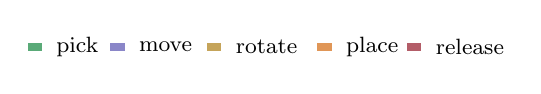
\begin{tikzpicture}[font=\rmfamily\fontsize{8}{8.8}\selectfont]
  \definecolor{gpick}{HTML}{5AAA78}
  \definecolor{gmove}{HTML}{8A86C8}
  \definecolor{grotate}{HTML}{C5A45A}
  \definecolor{gplace}{HTML}{E09657}
  \definecolor{grelease}{HTML}{B35D68}
  \foreach \x/\c/\t in {0/gpick/pick,1.05/gmove/move,2.28/grotate/rotate,
                          3.68/gplace/place,4.82/grelease/release}{
    \fill[\c] (\x,0) rectangle +(0.18,0.10);
    \node[anchor=west] at (\x+0.24,0.05) {\t};
  }
  \path[use as bounding box] (0,-0.08) rectangle (6.15,0.18);
\end{tikzpicture}


  \caption{Paired trajectories and execution timelines expose the localized
  response to each semantic event. (a) Task Update: the request changes to replace Mirinda with
  cola. (b) External Disturbance: the cola is moved to the other end of the
  conveyor during grasping. (c) Execution Failure: the conveyor moves too fast
  and both Franka manipulators fail their picks in succession. In each row,
  the left panel is the manipulator trajectory and the right panel is the
  corresponding Gantt chart.}
  \label{fig:gantt}
\end{figure}


\subsection{Experimental Setup}
\label{sec:experiment_setup}

The simulation uses the Isaac conveyor workspace in Fig.~\ref{fig:scenario}.
It contains heterogeneous manipulators, static and moving targets, global
visual observations, and a common primitive-skill interface. All methods use
the same scene and task assets, observations, success criterion, tracking and
safety stacks, and physical execution interface. Semantic calls use the LLM
\texttt{deepseek-ai/DeepSeek-V4-Flash} and the VLM
\texttt{Qwen/Qwen3.5-397B-A17B}. Conditions \texttt{C1}--\texttt{C4} cover
static and dynamic execution with task-relevant events \texttt{E1} (task
update), \texttt{E2} (external disturbance), and \texttt{E3} (verified
execution failure).
Each simulation condition contains 30 independent trials with randomly sampled
initial object layouts; events are injected at 30\%--70\% of subtask-completion
progress.
Evaluation uses task success, completion, efficiency, semantic reasoning, and
update-related metrics summarized in Tables~\ref{tab:baseline_tsr}--\ref{tab:hardware_results}
and the associated figures. Hardware conditions use 10 trials.

\subsection{Main Results}
\label{sec:main_results}

\begin{table}[t]
  \centering
  \caption{Baseline task success rate (TSR) over 30 trials across conditions.}
  \label{tab:baseline_tsr}
  \setlength{\tabcolsep}{2.0pt}
  \renewcommand{\arraystretch}{1.00}
  \scriptsize
  \begin{tabular*}{\columnwidth}{@{\extracolsep{\fill}}lcccccccc@{}}
    \toprule
    \multirow{2}{*}{\textbf{Method}} &
    \multirow{2}{*}{\textbf{C1}} &
    \multicolumn{3}{c}{\textbf{C2}} &
    \multirow{2}{*}{\textbf{C3}} &
    \multicolumn{3}{c}{\textbf{C4}} \\
    \cmidrule(lr){3-5}\cmidrule(lr){7-9}
    & & E1 & E2 & E3 & & E1 & E2 & E3 \\
    \midrule
    \textbf{Ours}
      & 30/30 & 30/30 & 30/30 & 30/30 & 27/30 & 30/30 & 30/30 & 27/30 \\
    End2End
      & 30/30 & 10/30 & 27/30 & 3/30 & 0/30 & 0/30 & 3/30 & 13/30 \\
    Agent per Robot
      & 10/30 & 3/30 & 13/30 & 17/30 & 3/30 & 0/30 & 0/30 & 0/30 \\
    COHERENT
      & 30/30 & 23/30 & 30/30 & 20/30 & 30/30 & 23/30 & 27/30 & 17/30 \\
    \bottomrule
  \end{tabular*}
\end{table}

\begin{figure}[!t]
  \centering
  \subfloat[SCR]{%
    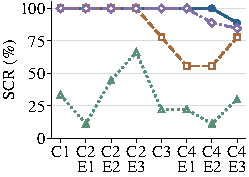
\includegraphics[width=.485\columnwidth]{figures/generated/figure5_a_scr.pdf}}
  \hfill
  \subfloat[Semantic reasoning time ratio]{%
    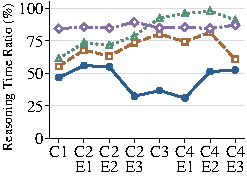
\includegraphics[width=.485\columnwidth]{figures/generated/figure5_b_reasoning_time.pdf}}
  \\[-1pt]
  \subfloat[Token usage]{%
    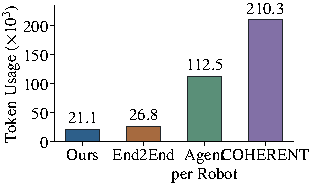
\includegraphics[width=.485\columnwidth]{figures/generated/figure5_c_token_usage.pdf}}
  \hfill
  \subfloat[Makespan]{%
    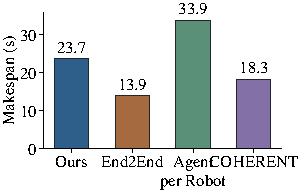
\includegraphics[width=.485\columnwidth]{figures/generated/figure5_d_makespan.pdf}}
  \\[-1pt]
  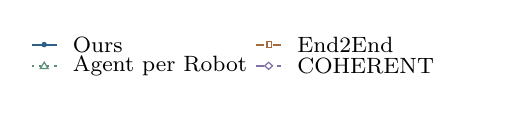
\begin{tikzpicture}[
    x=1cm,y=1cm,
    font=\rmfamily\fontsize{8}{8.8}\selectfont,
    legendline/.style={line width=.75pt}
  ]
    \definecolor{fours}{HTML}{2D5F8A}
    \definecolor{fend}{HTML}{A66A3F}
    \definecolor{fone}{HTML}{5A8F78}
    \definecolor{fcoh}{HTML}{8270A6}
    \draw[fours,legendline] (0,0)--(.32,0);
    \fill[fours] (.16,0) circle[radius=.035];
    \node[anchor=west] at (.40,0) {Ours};
    \draw[fend,legendline,dashed] (2.85,0)--(3.17,0);
    \draw[fend,line width=.45pt] (2.99,-.035) rectangle (3.05,.035);
    \node[anchor=west] at (3.25,0) {End2End};
    \draw[fone,legendline,dotted] (0,-.27)--(.32,-.27);
    \draw[fone,fill=white,line width=.45pt] (.16,-.225)--(.21,-.305)--(.11,-.305)--cycle;
    \node[anchor=west] at (.40,-.27) {Agent per Robot};
    \draw[fcoh,legendline,dash dot] (2.85,-.27)--(3.17,-.27);
    \draw[fcoh,fill=white,line width=.45pt]
      (3.01,-.225)--(3.06,-.27)--(3.01,-.315)--(2.96,-.27)--cycle;
    \node[anchor=west] at (3.25,-.27) {COHERENT};
    \path[use as bounding box] (-.05,-.38) rectangle (5.95,.12);
  \end{tikzpicture}
  \caption{Secondary event-handling metrics: (a) SCR, (b) semantic reasoning
  time ratio, (c) token usage, and (d) successful-trial makespan.}
  \label{fig:baseline_secondary}
\end{figure}



The proposed loop maintained high completion across all tested regimes while
changing only the event-relevant portion of the shared state. TSR was 30/30 in
the static, task-update, and disturbance conditions and 27/30 in the two
execution-failure conditions; SCR was 100\% except for 88.9\% in
\texttt{C4-E3}. The unsuccessful trials therefore occurred only under verified
execution-failure conditions rather than ordinary motion or task updates.
Figure~\ref{fig:event_graph_update} tracks the corresponding semantic-state
transitions. A task update revises $\gamma$ and the affected branches of $G$;
an external disturbance refreshes $\mathcal{F}$ and reconstructs branches whose
stored assumptions no longer hold; and an execution failure recorded in $z$
triggers repair of the failed node and its unfinished dependencies. In each
case, $\mathcal{N}_k^{\mathrm{aff}}$ is identified, unaffected valid nodes are
retained, and only the affected subgraph is reconstructed, providing
qualitative evidence of selective update.

The paired trajectories and timelines in Fig.~\ref{fig:gantt} show how this
design is realized. Verified independent nodes are dispatched together, local
tracking handles continuous target motion, and semantic reasoning is invoked
only at initialization, verification boundaries, or task-relevant events. The
reported time, makespan, and token ranges quantify this trade-off; the larger
token cost in \texttt{C4-E3} is consistent with its additional verified repair
branch.

\subsection{Comparison with Baselines}
\label{sec:baseline_comparison}

The comparison uses the same task, observations, capabilities, primitive
skills, trial count, and success criterion for every method. \textbf{End2End} directly
maps the task and observation to commands without the shared semantic state.
\textbf{Agent per Robot} gives each manipulator an independent language-model agent,
whereas \textbf{COHERENT} adapts the heterogeneous multi-robot collaboration protocol
of Liu~\emph{et al.}~\cite{liu2025coherent} to the same interface.

\begin{figure}[!t]
  \centering
  \newcommand{\failurePanel}[3]{%
  \begin{minipage}[t]{.485\columnwidth}
    \centering
    \includegraphics[width=\linewidth]{#1}
    \vspace{0.10em}
    {\scriptsize\textbf{(#2) #3}\par}
  \end{minipage}}

\failurePanel{figures/figure6/a.pdf}{a}{Invalid capability}
\hfill
\failurePanel{figures/figure6/b.pdf}{b}{Execution anomaly}
\vspace{0.35em}

\failurePanel{figures/figure6/c.pdf}{c}{Assignment conflict}
\hfill
\failurePanel{figures/figure6/d.pdf}{d}{Task timeout}

  \caption{Representative failures: (a) invalid workspace capability, (b)
  collision, (c) conflicting assignment, and (d) timeout after repeated
  replanning.}
  \label{fig:failure_analysis}
\end{figure}

\begin{figure}[!t]
  \centering
  % Generated PDF source:
% figures/generate_figure6_failure_distribution.py reads tables/failure.xlsx.
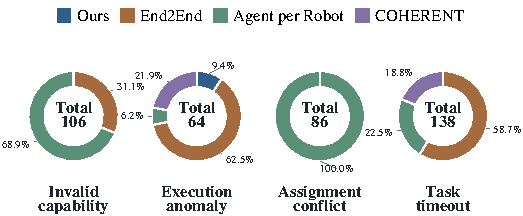
\includegraphics[width=\columnwidth]{figures/generated/figure6_e_failure_distribution.pdf}

  \vspace{-0.1in}
  \caption{Failure counts and baseline proportions by failure type.}
  \label{fig:failure_distribution}
\end{figure}


Ours retained 30/30 on all task-update
and disturbance cases and 27/30 under execution failure, while every baseline
lost substantially more event trials.
Table~\ref{tab:baseline_tsr} reports their
condition-wise TSR, making the event-specific gap below directly comparable.
The largest gap occurred when semantic events had to be incorporated.
In static \texttt{C1}, all methods except
Agent per Robot obtained 30/30, isolating the difference to event-aware
coordination rather than the basic skill interface.
The secondary metrics in Fig.~\ref{fig:baseline_secondary} show the same
ordering: among the compared methods, Ours had the highest event-condition SCR
and the lowest semantic-time ratio and token use. Ours had a longer
successful-trial makespan than End2End but higher event-condition completion.


\begin{figure*}[!t]
  \centering
  \newcommand{\figsevenframe}[1]{%
  \includegraphics[width=.188\textwidth]{figures/figure8/#1.jpg}}

\setlength{\tabcolsep}{1.1pt}
\renewcommand{\arraystretch}{0.92}
\begin{tabular}{@{}l@{\hspace{.35em}}ccccc@{}}
  \multicolumn{6}{@{}l}{\footnotesize\textbf{(a)} \texttt{H1} Normal cooperative execution: observe $\rightarrow$ assign $\rightarrow$ execute $\rightarrow$ place}
  \\[-1pt]
  & \figsevenframe{a-1} & \figsevenframe{a-2} & \figsevenframe{a-3}
  & \figsevenframe{a-4} & \figsevenframe{a-5} \\
  \multicolumn{6}{@{}l}{\footnotesize\textbf{(b)} \texttt{H2} Task update adaptation: execute current plan $\rightarrow$ update $\gamma$ $\rightarrow$ revise affected branch $\rightarrow$ continue execution}
  \\[-1pt]
  & \figsevenframe{c-1} & \figsevenframe{c-2} & \figsevenframe{c-3}
  & \figsevenframe{c-4} & \figsevenframe{c-5} \\
  \multicolumn{6}{@{}l}{\footnotesize\textbf{(c)} \texttt{H3} External disturbance recovery: approach target $\rightarrow$ human disturbance $\rightarrow$ verify inconsistency $\rightarrow$ recover downstream pick}
  \\[-1pt]
  & \figsevenframe{b-1} & \figsevenframe{b-2} & \figsevenframe{b-3}
  & \figsevenframe{b-4} & \figsevenframe{b-5} \\
\end{tabular}

  \vspace{-0.1in}
  \caption{Hardware sequences provide verification evidence for normal motion,
  task update, and external disturbance.}
  \label{fig:hardware_experiments}
\end{figure*}

\subsection{Failure Analysis and Ablation Study}
\label{sec:failure_analysis}
\label{sec:ablation}

\subsubsection{Cause of Task Failures}


The failure counts in Fig.~\ref{fig:failure_distribution} quantify the
intermediate coordination state. Ours had no capability, assignment, or timeout
failures and only six physical execution anomalies, whereas the baselines
exhibited the corresponding semantic failures. Fig.~\ref{fig:failure_analysis}
shows representative cases: role ownership filters invalid dispatches and
verification exposes residual physical anomalies for repair.

\subsubsection{Key Ablations}

\begin{table}[t]
  \centering
  \caption{Ablation TSR, SCR and Reasoning Time under
  \texttt{C4} (30 trials).}
  \label{tab:ablation_comparison}
  \setlength{\tabcolsep}{1.25pt}
  \renewcommand{\arraystretch}{1.00}
  \scriptsize
  \begin{tabular*}{\columnwidth}{@{\extracolsep{\fill}}lccccccccc@{}}
    \toprule
    \multirow{2}{*}{\textbf{Method}} &
    \multicolumn{3}{c}{\textbf{E1}} &
    \multicolumn{3}{c}{\textbf{E2}} &
    \multicolumn{3}{c}{\textbf{E3}} \\
    \cmidrule(lr){2-4}\cmidrule(lr){5-7}\cmidrule(lr){8-10}
    & {\fontsize{6.3}{6.8}\selectfont TSR}
    & {\fontsize{6.3}{6.8}\selectfont SCR}
    & {\fontsize{6.3}{6.8}\selectfont Time}
    & {\fontsize{6.3}{6.8}\selectfont TSR}
    & {\fontsize{6.3}{6.8}\selectfont SCR}
    & {\fontsize{6.3}{6.8}\selectfont Time}
    & {\fontsize{6.3}{6.8}\selectfont TSR}
    & {\fontsize{6.3}{6.8}\selectfont SCR}
    & {\fontsize{6.3}{6.8}\selectfont Time} \\
    \midrule
    \textbf{Ours}
      & \textbf{30/30} & \textbf{100} & \textbf{.309}
      & \textbf{30/30} & \textbf{100} & \textbf{.513}
      & \textbf{27/30} & 88.9 & \textbf{.525} \\
    \shortstack[l]{w/o Role\\Separation}
      & 23/30 & 82.1 & .462
      & \textbf{30/30} & \textbf{100} & .567
      & 0/30 & 78.2 & .796 \\
    \shortstack[l]{w/o Selective\\Replanning}
      & 26/30 & \textbf{100} & .456
      & \textbf{30/30} & \textbf{100} & .545
      & 17/30 & \textbf{93.0} & .658 \\
    \bottomrule
  \end{tabular*}
\end{table}


\begin{figure}[!t]
  \centering
  % Generated PDF source:
% The generator reads tables/failure.xlsx and produces the manuscript's Figure 8.
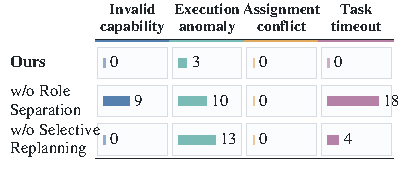
\includegraphics[width=\columnwidth]{figures/generated/figure7_ablation_failure_count.pdf}

  \vspace{-0.1in}
  \caption{Ablation failure counts under \texttt{C4}. A1 and A2 denote the
  variants without role separation and selective replanning, respectively.}
  \label{fig:ablation_failure_count}
\end{figure}


\begin{table}[t]
  \centering
  \caption{Hardware results over 10 trials. Resp. is event-response time (s);
  Aff./Pend. is the affected-to-pending node ratio.}
  \label{tab:hardware_results}
  \small
  \setlength{\tabcolsep}{2.8pt}
  \begin{tabular}{lcccc}
    \toprule
    Condition & TSR & SCR (\%) & Resp. (s) & Aff./Pend. \\
    \midrule
    \texttt{H1} Normal
      & 10/10 & 100.0 & --   & --   \\
    \texttt{H2} Task Update
      & 9/10  & 98.6  & 11.3 & 0.38 \\
    \texttt{H3} External Disturbance
      & 7/10  & 92.3  & 9.7  & 0.14 \\
    \bottomrule
  \end{tabular}
\end{table}

\begin{figure}[t]
  \centering
  \setlength{\tabcolsep}{.5pt}
  \begin{tabular}{@{}lccc@{}}
    \raisebox{8pt}{%
      \shortstack[r]{%
        \fontsize{8}{9}\selectfont L. Franka\\[3pt]
        \fontsize{8}{9}\selectfont R. Franka\\[3pt]
        \fontsize{8}{9}\selectfont Ranger}} &
    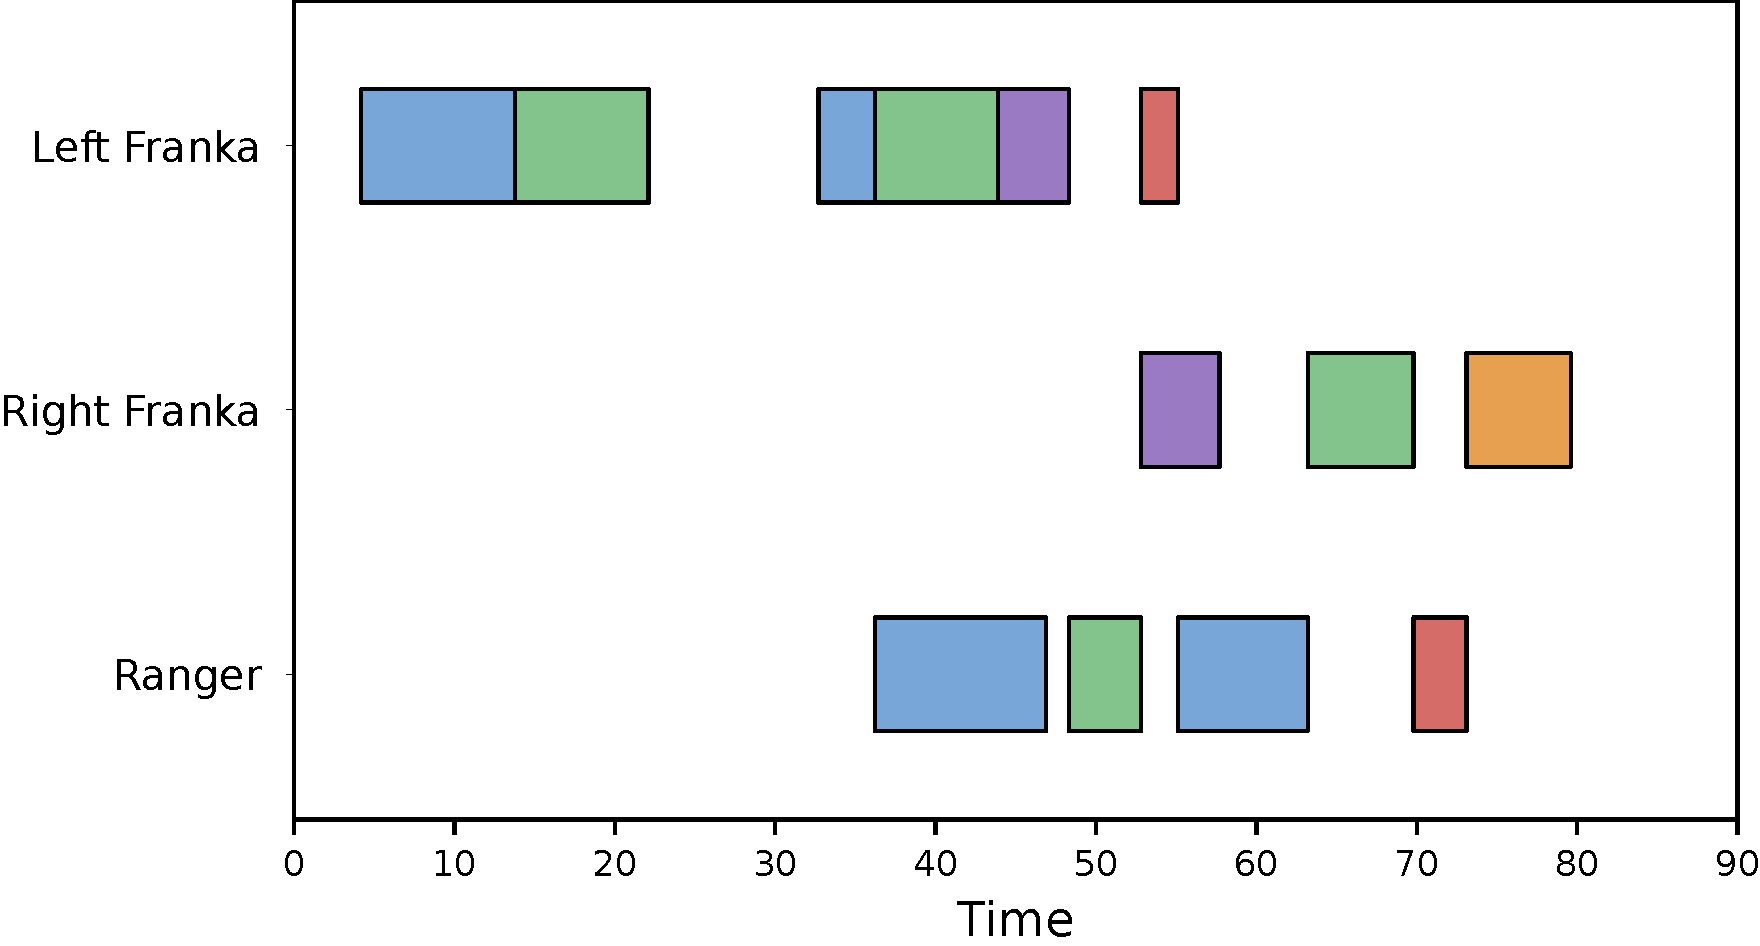
\includegraphics[trim=126pt 28pt 0 0,clip,width=.27\columnwidth]{figures/figure_new/a.pdf} &
    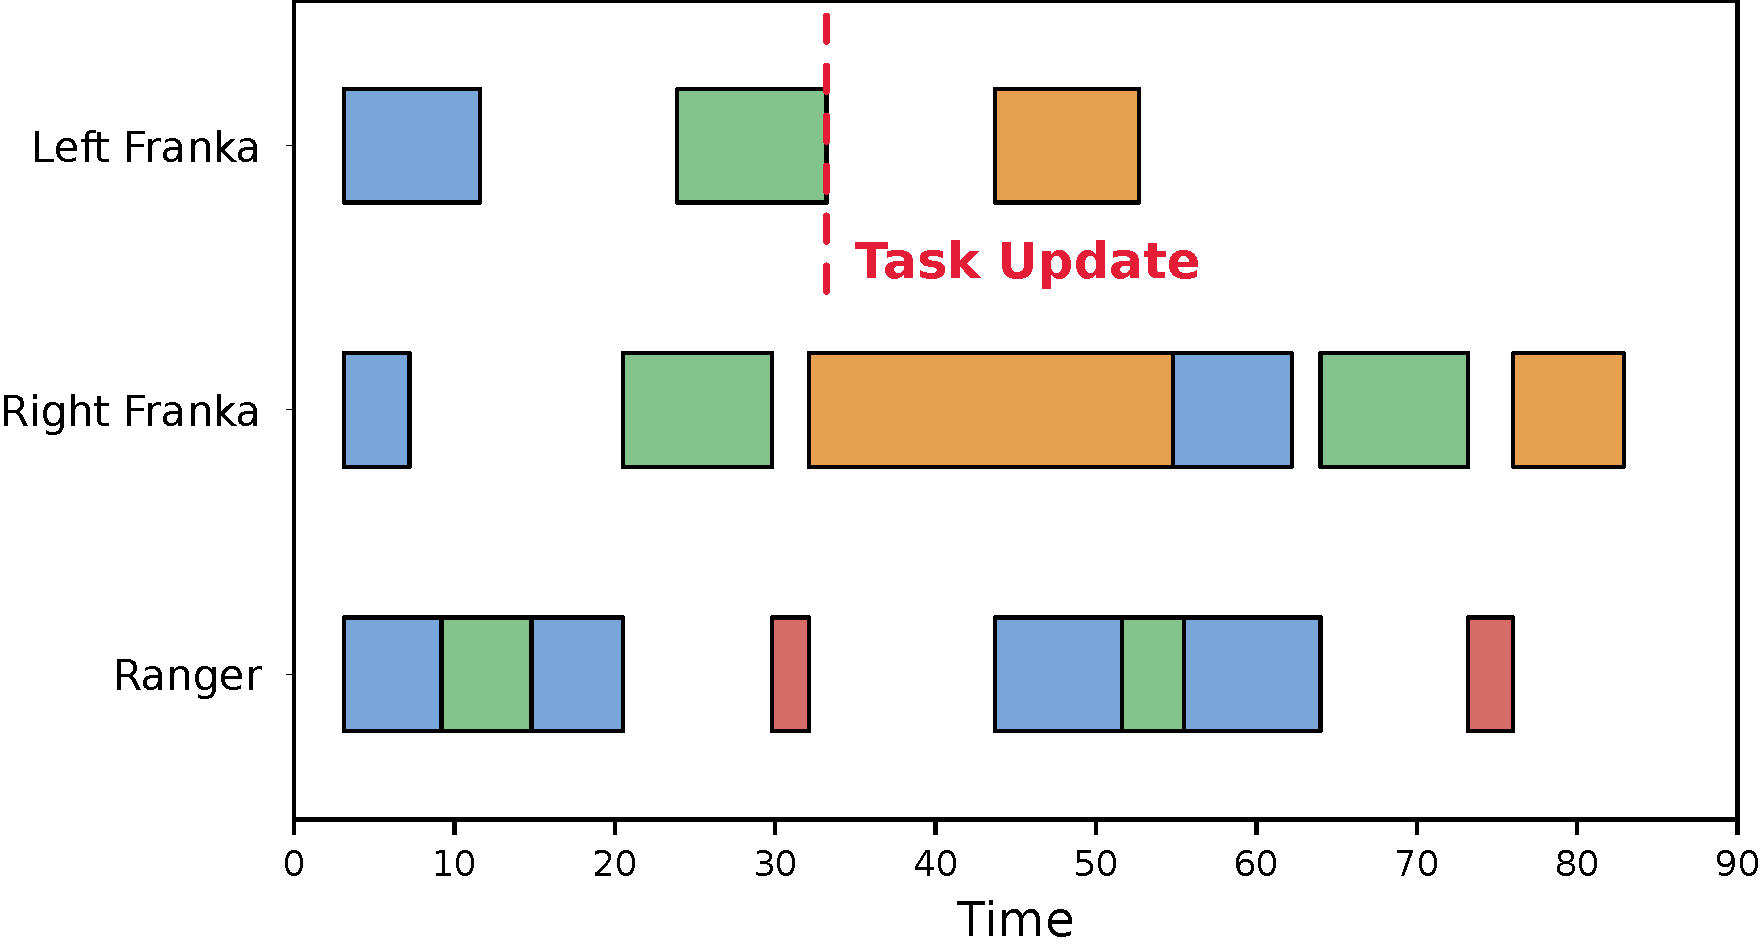
\includegraphics[trim=126pt 28pt 0 0,clip,width=.27\columnwidth]{figures/figure_new/b.pdf} &
    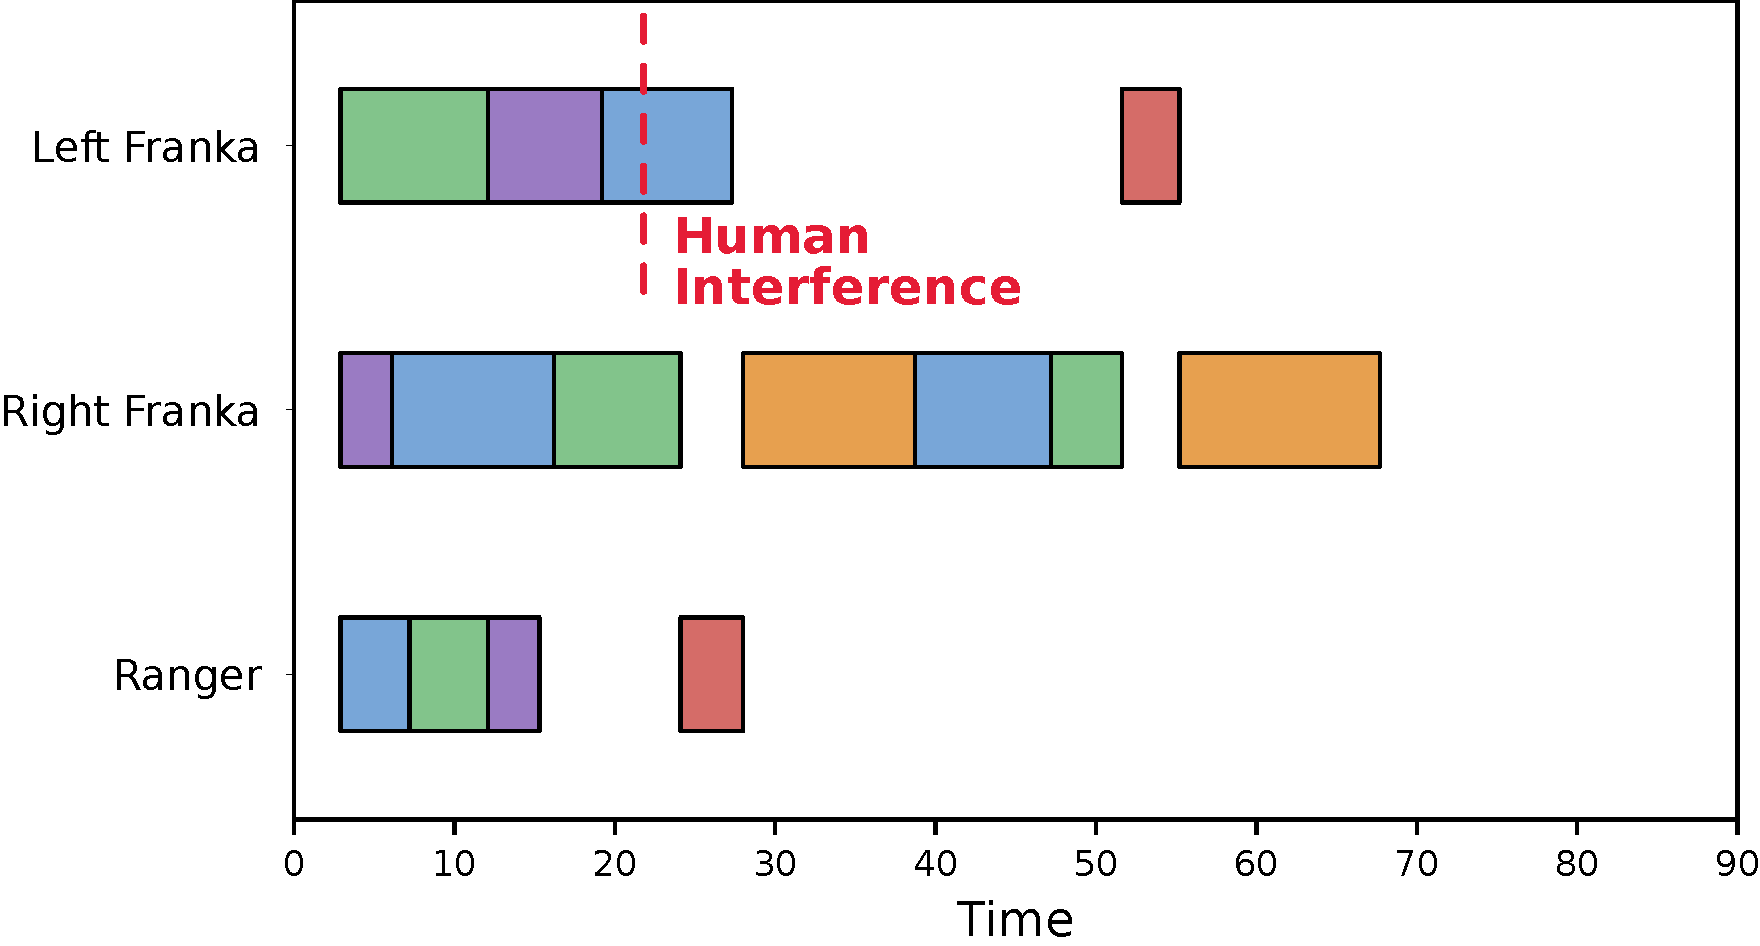
\includegraphics[trim=126pt 28pt 0 0,clip,width=.27\columnwidth]{figures/figure_new/c.pdf}
  \end{tabular}

  \vspace{1pt}
  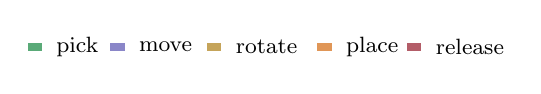
\begin{tikzpicture}[font=\rmfamily\fontsize{8}{8.8}\selectfont]
  \definecolor{gpick}{HTML}{5AAA78}
  \definecolor{gmove}{HTML}{8A86C8}
  \definecolor{grotate}{HTML}{C5A45A}
  \definecolor{gplace}{HTML}{E09657}
  \definecolor{grelease}{HTML}{B35D68}
  \foreach \x/\c/\t in {0/gpick/pick,1.05/gmove/move,2.28/grotate/rotate,
                          3.68/gplace/place,4.82/grelease/release}{
    \fill[\c] (\x,0) rectangle +(0.18,0.10);
    \node[anchor=west] at (\x+0.24,0.05) {\t};
  }
  \path[use as bounding box] (0,-0.08) rectangle (6.15,0.18);
\end{tikzpicture}

\vspace{-0.1in}
  \caption{Hardware timelines for Fig.~\ref{fig:hardware_experiments}: left,
  normal motion; middle, task-update revision; right, disturbance recovery.}
  \label{fig:hardware_gantt}
\end{figure}



Under \texttt{C4}, the ablations remove role ownership or selective replanning.
Table~\ref{tab:ablation_comparison} shows lower event TSR for both, most under
execution failure. Role-ablation errors in
Fig.~\ref{fig:ablation_failure_count} support this attribution: the
role-separated design limits error propagation by assigning each updated
semantic component a dedicated owner, namely affordance for $\mathcal{F}$,
planning for $G$, and verification for $z$. Without selective replanning,
higher semantic-time ratios show that semantic reasoning occupies more of the
execution horizon. Together with the lower event TSR, this result associates
selective replanning with lower semantic reasoning occupancy and better task
progress under the tested events.

\subsection{Hardware Experiments}
\label{sec:hardware_experiments}

The hardware platform contains two fixed Franka manipulators and a third
manipulator on an AgileX Ranger Mini V2. An AgileX SCOUT MINI carries task
objects as a teleoperated moving carrier; it is not a semantic coordinator.
The same shared state, primitive-skill interface, and event update path are
used on hardware. Each condition is repeated for 10 trials.
Figure~\ref{fig:hardware_role_outputs} exposes the role-level semantic updates
for the task-update and disturbance trials. In the top row, the revised
instruction enters $\gamma$, the affordance role refreshes $\mathcal{F}$, the
verification role identifies the affected nodes, and the planning role revises
$G$ while retaining unaffected work. The object relocation
refreshes $\mathcal{F}$, verification records the failed execution status in
$z$ and traces the invalidated dependencies, and planning repairs the affected
branch of $G$. The three role outputs are committed together as the
corresponding update of $S_{\mathrm{sem}}$ before dispatch resumes.




\begin{figure}[!t]
  \centering
  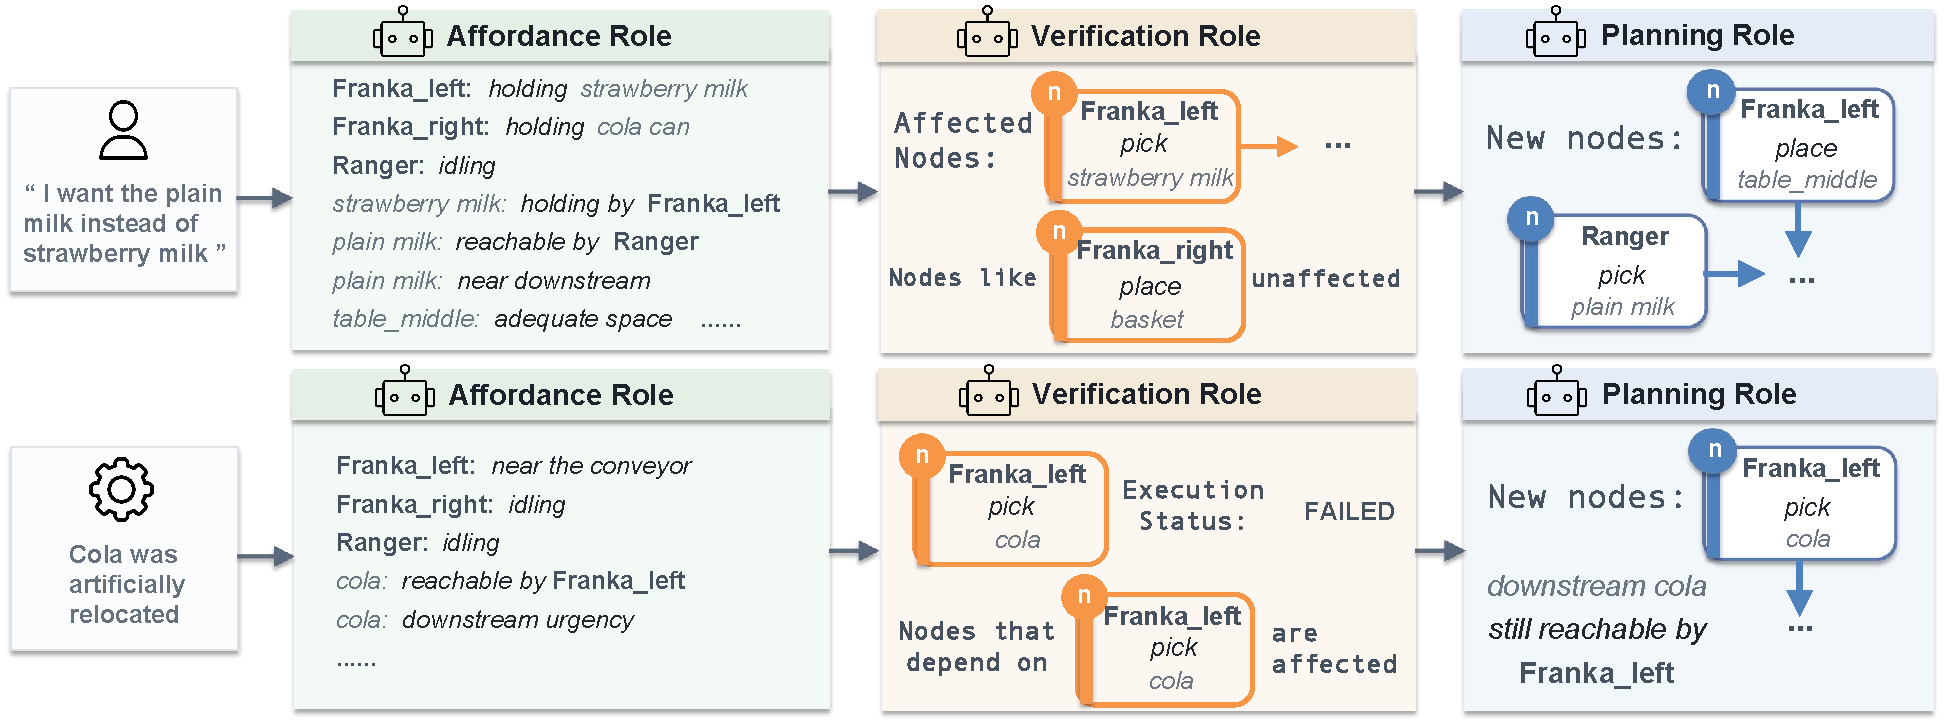
\includegraphics[width=\columnwidth]{figures/figure_role/figure_role.pdf}
  \caption{Intermediate outputs of the affordance, verification, and planning
  roles after the task-update event in the middle panel of
  Fig.~\ref{fig:hardware_gantt} (\textbf{Top}) and the external disturbance in the
  right panel (\textbf{Bottom}).}

  \label{fig:hardware_role_outputs}
\end{figure}


The three scenarios isolate normal motion, a task update, and a disturbance.
Table~\ref{tab:hardware_results} reports 10/10 TSR and 100.0\% SCR for
\texttt{H1}, 9/10 and 98.6\% for \texttt{H2} (11.3 s response, 0.38
affected/pending), and 7/10 and 92.3\% for \texttt{H3} (9.7 s, 0.14).
The recorded traces show that semantic updates are committed online before
dispatch resumes rather than reconstructed after a run: H2 updates $\gamma$
after the instruction change, H3 refreshes $\mathcal{F}$ after the disturbance,
and verification updates $z$ at execution boundaries. In H3, the resulting
revision covers a 14\% affected scope while retaining unaffected work. These
physical executions therefore corroborate the online update sequence; the
lower H3 TSR also shows that selective updating does not eliminate physical
uncertainty.

% \input{sections/limitations.tex}
\section{Conclusion}
\label{sec:conclusion}

This work proposes role-shared semantic coordination for dynamic heterogeneous
multi-arm manipulation with continual physical changes. The framework assigns
explicit semantic responsibilities to the affordance, planning, and
verification roles over a shared semantic state, and uses event-driven
selective updates to reconsider only the affected scope after task updates,
external disturbances, or execution failures. Within the tested heterogeneous
manipulation scenarios, baseline, ablation, and hardware results support role
separation for semantic responsibility allocation and selective updates for
efficient adaptation under semantic events.
The framework coordinates semantic decisions and semantic-state updates; it
does not replace local skill controllers, perception, low-level control, or
physical execution modules. The remaining execution boundary is visible in the
27/30 success rate for simulation execution failures and the 7/10 success rate
for the hardware disturbance condition, where physical uncertainty can still
prevent completion.


\bibliographystyle{IEEEtran}
\bibliography{references}

\end{document}
